\chapter{Обзор методов обучения с подкреплением и их применения в роботике}\label{ch:ch1}

Машинное обучение с подкреплением строится на взаимодействии агента со средой. Средой в зависимости от решаемой задачи может являться компьютерная игра, мир окружающий робота или физическая установка. Граница разделяющая агента и среду достаточно условна. В качестве примера можно рассмотреть робот-манипулятор. Если агент непосредственно управляет положением суставов манипулятора, то суставы является частью агента. Если же агент задает конечное положение захвата манипулятора, а положение составов вычисляется с помощью встроенного алгоритма, то суставы манипулятора являются частью среды. 

Агент взаимодействует со средой посредством совершения  действий из заранее заданного набора $a \in \mathcal{A}$. При каждом действии агента среда переходит в новое состояние $s^{\prime} \in \mathcal{S}$, а агент получает награду $r \in \mathcal{R}$.
Цель обучения агента заключается в нахождении такой последовательности действий, при которой агент получит максимальную суммарную награду.

\section{Обзор методов глубокого обучения с подкреплением}\label{sec:ch1/sec1}

Глубокое обучение с подкреплением основано на объединении нейронных сетей и методов обучения с подкреплением. Нейронная сеть в этом случае выступает в качестве универсального аппроксиматора и определяет стратегию агента при взаимодействии со средой $\pi_{\theta}$.

\subsection{Нейронные сети}

Понятие искусственной нейронной сети было впервые предложено У. Маккалоком и У. Питтсом в 1943 году в работе "Логическое исчисление идей, относящихся к нервной активности" \cite{McCulloch1943}. Первая нейронная сеть с одним скрытым слоем, пороговой функцией активации и прямым распространением сигнала была предложена Ф. Розенблаттом в 1957 году \cite{rosenblatt}.

\begin{figure}[ht]
	\centerfloat{
		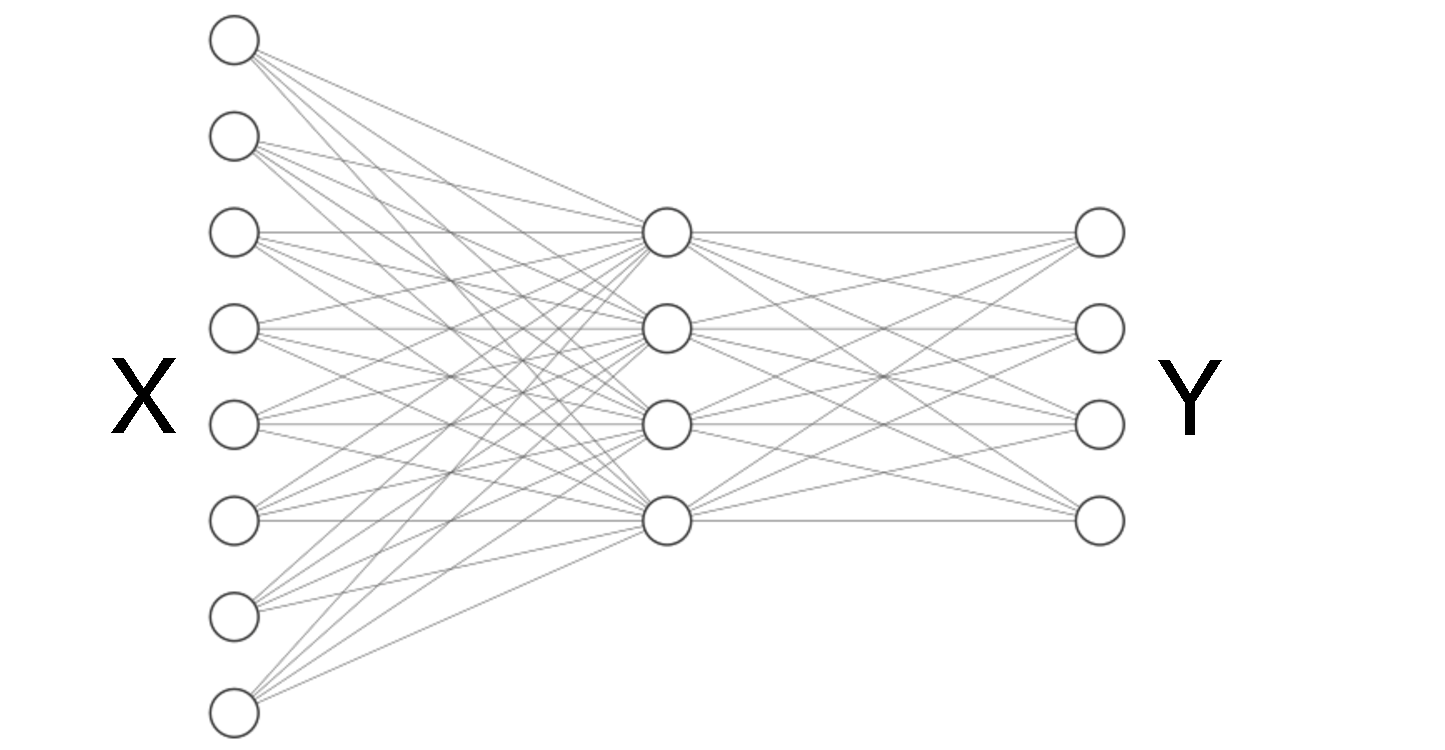
\includegraphics[width=0.7\linewidth]{images/fcnn}
	}
	\caption{Полносвязная нейронная сеть с одним скрытым слоем}
	\label{fig:fcnn}
\end{figure}

Схематически полносвязная нейронная сеть с одним скрытым слоем представлена на рис. \ref{fig:fcnn}. Нейронная сеть принимает на вход вектор входных параметров $X$ и возвращает на выходе вектор выходных параметров $Y$. Значение в нейроне на слое $i$ вычисляется как взвешенная сумма значений нейронов на слое $i - 1$ плюс смещение (bias). Таким образом значения получаемые в нейронах на слое $i$ можно представить в виде $x_i = \sigma(W_{nm} \cdot x_{i - 1} + b_m)$, где $\sigma$ - функция активации, $W_{nm}$ - матрица весов, $b_m$ - вектор смещений, $x_{i - 1}: |x_{i - 1}| = m$ - значения активаций на слое $i - 1$, а $x_{i}: |x_{i}| = n$ - значения активаций на слое $i$. Для оптимизации (обучения) параметров нейросети применяется алгоритм обратного распространения ошибки, который был одновременно разработан А.И. Галушкиным \cite{Galushkin} и П.Д.Вебросом \cite{webros_1974}. На каждой итерации алгоритма \ref{alg:backprop} происходит два прохода - прямой и обратный. Во время прямого прохода ($X \to Y$) вычисляются выходные значения при прохождении входного вектора от входов сети к выходам. Затем во время обратного прохода ошибка предсказания для слоя $i$ вычисляется на основе ошибки для слоя $i + 1$ и обновление весов производится с помощью метода градиентного спуска. 

\begin{algorithm}[ht]
	\SetAlgoLined
	\KwIn{$X$ - входные наблюдения, $\hat{Y}$ - ожидаемые выходные значения, $L(Y, \hat{Y})$ - функция потерь, $W$ - параметры нейронной сети}
	\KwOut{$W^{\prime}$ - новые значения параметров нейронной сети}
	\While{$L(Y, \hat{Y})$ > $\varepsilon$}{
		Выбираем $x \sim X$, $\hat{y} \sim \hat{Y}$\;
		Прямой проход: y = NN(W, x)\;
		Вычисляем ошибку предсказания: $E = L(y, \hat{y})$\;
		Обратный проход: 
		$\Delta w_{ij} = -\alpha \frac{\partial E}{\partial w_{ij}}$\;
		$S_j = \sum_{i = 1}^{n}w_{ij}x_i$\;
		$\frac{\partial E}{\partial w_{ij}} = \frac{\partial E}{\partial S_j}\frac{\partial S_j}{\partial w_{ij}} = x_i\frac{\partial E}{\partial S_j}$\;
		
	}
	\caption{Алгоритм обратного распространения ошибки}
	\label{alg:backprop}

\end{algorithm}

Нейронные сети получили широкое распространение в самых разных задачах таких как распознавание изображений \cite{alexnet} и анализ текстов на естественном языке \cite{bert} благодаря тому, что нейронная сеть с достаточно большим количеством параметров может выступать в качестве универсального аппроксиматора. Частичным доказательством этого утверждения является теорема Колмогорова-Арнольда\cite{kolmogorov, arnold} доказывающая, что многомерная функция многих переменных может быть представлена в виде суперпозиции непрерывных функций одной переменной. 

\subsection{Обучение с подкреплением}

Принципиальная схема обучения RL алгоритмов приведена на рисунке \ref{fig:rl}. На ней RL агент взаимодействуя со средой получает от нее состояние (s $\in \mathcal{S}$), награду ($r: \mathcal{S} \times \mathcal{A} \to \mathbb{R}$), и флаг завершения эпизода (done $\in \{0, 1\}$).  В среде агент совершает действие ($a \in \mathcal{A}$) которое переводит среду в следующее состояние ($s^{\prime} \in \mathcal{S}$). В зависимости от того является ли переход из состояния $s$ в состояние $s^{\prime}$ при действии $a$ единственным или одним из возможных с распределением $p(s^{\prime},r|s,a)$, среда называется детерминированной или не детерминированной. 

\begin{figure}[ht]
	\centerfloat{
		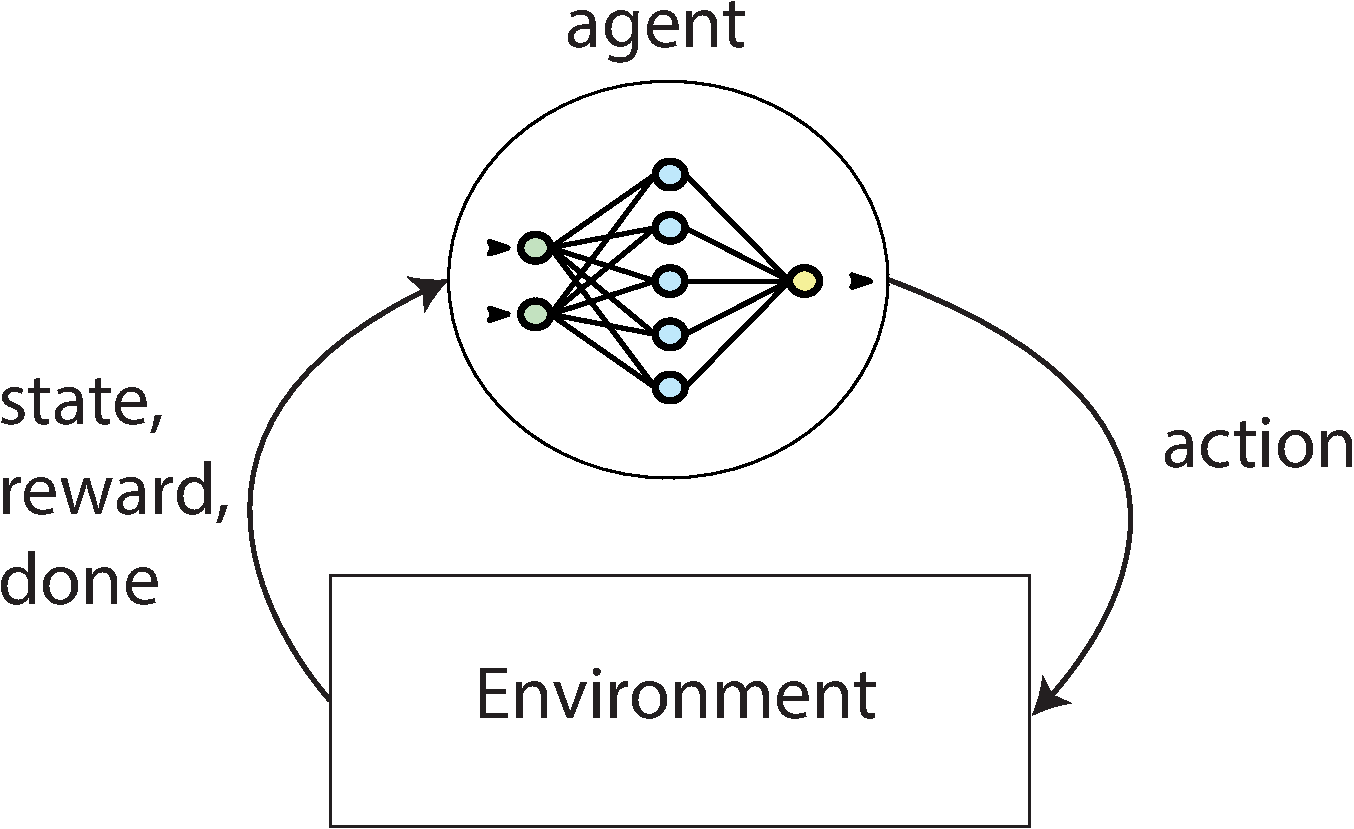
\includegraphics[width=0.5\linewidth]{images/rl_setting}
	}
	\caption{Взаимодействие агента и среды}
	\label{fig:rl}
\end{figure}

Взаимодействие RL агента со средой происходит в рамках марковского процесса принятия решений (МППР). В нем предполагается, что следующее состояние и награда получаемая агентом зависит (детерминировано или стохастически) только от предыдущего состояния и действия которое агент совершил. Если же у среды есть некоторые не наблюдаемые параметры, то говорят о частично наблюдаемом марковском процессе принятия решений (ЧНМППР). В нем наблюдение в момент времени $t$ --- $o_t \in \mathcal{O}$ определяется распределением $o_t \sim p(o_t|s_t)$, где $s_t \in \mathcal{S}$ полное состояние среды. 

Стратегия агента задается функцией $a_t=\pi(s_t)$ отображающей пространство состояний (наблюдений) в пространство действий $\mathcal{A}$. Стратегия агента может быть как детерминированной, так и стохастической. Задача агента состоит в максимизации суммарной ожидаемой дисконтированной награды к концу эпизода:

\begin{equation}
\ex_{\tau \sim \pi_{\theta}} [J(\tau)] = \ex_{\tau \sim \pi_{\theta}} [r_0 + \gamma r_{1} + \gamma ^ 2 r_{2} + ...] = \ex_{\tau \sim \pi_{\theta}} [\sum_{t} \gamma ^t r_{t}]
\end{equation}

Коэффициент $\gamma \in (0, 1]$ вводится для  ограничения эффективного горизонта --- числа шагов при котором будущая награда не влияет на стратегию из-за дисконтирования ($\gamma ^ n r$). Он также позволяет регулировать уровень жадности агента --- на сколько награда получаемая на текущем шаге ценнее аналогичной награды получаемой на следующем шаге. Математическое ожидание берется по траекториям $\tau$ полученным с помощью текущей стратегии $\pi_{\theta}$ параметризованной весами $\theta$. 
Вероятность траектории $\tau$ может быть записана следующим образом:
 
 \begin{equation}
     p(\tau|\pi) = p(s_0) \prod^T_{t=1}p(s_t|s_{t-1}, a_{t-1})\cdot \pi(a_{t-1}, s_{t-1})
\end{equation}

 где $p(s_0)$ - распределение начальных состояний в каждом эпизоде, $p(s_t|s_{t-1}, a_{t-1})$ - распределение описывающее динамику среды. Таким среда однозначно задается множеством состояний $\mathcal{S}$, действий $\mathcal{A}$, наград $\mathcal{R}$, динамикой переходов $\mathcal{R}$ и параметром $\gamma$ --- $<\mathcal{S, A, R, P}, \gamma>$.


\subsection{Уравнение Беллмана}

Ценность нахождения агента в текущем состоянии $s_t$ описывается с помощью V-функции и связанной с ней Q-функции. $V(s_t) = \ex[\sum \gamma ^t r_{t}]$ оценивает суммарную дисконтированную награду, которую получит агент находящийся в состоянии $s_t$ если он будет действовать согласно текущей стратегии. $Q(s_t, a_t) = \ex[r_t + \sum \gamma ^{t + 1} r_{t + 1}]$ оценивает суммарную дисконтированную награду, которую получит агент при совершении действия $a_t$ в состоянии $s_t$ при условии, что дальше он будет следовать текущей стратегии. С помощью V-функции можно сравнивать между собой две различные стратегии --- стратегия $\pi^{\prime}$ лучше стратегии $\pi$ если ожидаемая награда для первой стратегии $V_{\pi^{\prime}} \geq V_{\pi}$ для всех $s \in \mathcal{S}$. Таким образом можно определить оптимальную стратегию $\pi^*: V_{\pi^*} \geq  V_{\pi} \  \forall \pi$. Значения V, Q-функций в точках $s_t$ и $s_{t + 1}$ при условии, что текущая стратегия является оптимальной связаны между собой уравнениями Беллмана: 

\begin{equation}
	V^*(s) = \max_{a \in \mathcal{A}} \ex(r_{t + 1} + \gamma V^*(s_{t + 1}))
\end{equation}

\begin{equation}
Q^*(s, a) = \ex(r_{t + 1} + \gamma \max_{a' \in \mathcal{A}} Q^*(s_{t + 1}, a'))
\end{equation}

Значения оптимальных V, Q-функций связаны между собой: 

\begin{equation}
V^*(s) = \max_{a \in \mathcal{A}}Q^*(s, a)
\end{equation}

Смысл V-функции можно легко интерпретировать в задаче изображенной на рис. \ref{fig:minigrid}. В ней агент движется из верхнего левого угла ($s_0$) сетки в правый нижний угол ($s_f$). Если агент за каждый шаг получает награду $r = -1$, то оптимальная V-функция при условии того, что коэффициент дисконтирования $\gamma = 1$ в состоянии $s_t$ будет равна числу действий необходимых для достижения состояния $s_f$ взятых со знаком ``-''. 

\begin{figure}[ht]
	\centerfloat{
		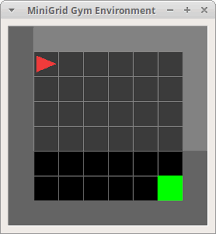
\includegraphics[width=0.3\linewidth]{images/minigrid_empty}
	}
	\caption{Среда MiniGrid-Empty-8x8-v0 \cite{gym_minigrid}}
	\label{fig:minigrid}
\end{figure}

 
\subsection{Метод value iteration}

Уравнения Беллмана могут быть использованы для построения оптимальной стратегии для сред с конечным набором состояний и известным распределением переходов между ними $p(s^{\prime}, r|s, a)$. Метод value iteration \ref{alg:value_it} строится на применении метода простой итерации к уравнению Беллмана для V-функции. Данный метод имеет гарантированную сходимость \cite{Sutton1998}, но может быть использован только для очень ограниченного набора задач.

\begin{algorithm}[ht]
	\SetAlgoLined
	\KwIn{$t$ - условие останова, $\mathcal{S}$ - набор состояний среды, $p(s^{\prime}, r|s, a)$ - распределение вероятности переходов}
	\KwOut{$\pi(s) = \mathrm{argmax}_{a} \sum_{s', r}p(s',r|s,a)[r + \gamma V(s')]$}
	Инициализируем V(s) = 0 (для всех $s \in \mathcal{S}$), $\Delta = \infty$\;
	\While{$\Delta$ > t}{
		$\Delta$ = 0\;
		\ForEach{s $\in \mathcal{S}$}{
		    $V_{old}$ = V(s)\\
		    %V_{old}(s) = V(s)\par
			V(s) = $\max_a \sum_{s', r}p(s', r|s, a)[r + \gamma V(s')]$\\
			$\Delta = \max(\Delta, |V_{old} - V(s)|)$
		}
	}
	\caption{Алгоритм value iteration}
	\label{alg:value_it}

\end{algorithm}

В рамках данной работы были использованы алгоритмы глубокого обучения с подкреплением обучающиеся методом проб и ошибок и не строящие в явном виде моделей награды и переходов среды. В зависимости от того, как используются данные полученные от среды такие алгоритмы можно разделить на два больших класса on-policy и off-policy. В on-policy алгоритмах агент обучается на данных полученных с помощью текущей стратегии. Благодаря этому получается добиться большей стабильности обучения, но требуется гораздо больше данных так как нет возможности переиспльзовать данные полученные при взаимодействии устаревшей стратегии со средой. 
В off-policy алгоритмах агент выучивает оптимальную стратегию (Q-функцию) используя исторические данные взаимодействия со средой полученные при использовании предыдущих версий стратегии. 

\subsection{Off-policy алгоритмы}

\paragraph{Алгоритм DQN}

Одними из наиболее популярных методов основанных на приближенном вычислении Q-функции являются алгоритмы Q-learning \cite{Watkins_1992} и Deep Q-learning \cite{mnih2013atari}. В методе Q-learning функция $Q(s, a)$ иттеративно обновляется на основании опыта собранной текущей стратегией. В работе \cite{SuttonQLearning} показано, что функция обновляемая таким методом сходится к оптимальной Q-функции.

Существенный прорыв в методах основанных на Q-обучении был достигнут в 2015 году. Благодаря использованию нейронных сетей в качестве аппроксиматора для Q-функции авторами \cite{mnih2013atari} был разработан метод DQN который обучился играть в 49 игр Atari на уровне человека. Игры Atari рассматриваются в качестве одного из основных тестов для сравнения качества работы различных алгоритмов основанных на глубоком обучении с подкреплением.  

Алгоритм DQN строится на обучении глубокой нейронной сети аппроксимировать Q-функцию для каждого возможного действия в зависимости от текущего состояния игры --- изображения или последовательности изображений 84x84 пикселя. Для стабилизации процесса обучения Q-функции авторы использовали следующее выражение для функции потерь:

\begin{equation}
    L(\theta) = \ex_{<s, a, r, s^{\prime}> \sim \mathcal{D}}\left[\left(r + \gamma \max_{a^{\prime}}
    Q_{\theta^-(s^{\prime}, a^{\prime})} - Q_{\theta}(s, a)\right)^2 \right]
\label{eq:dqn}
\end{equation}

Буфер $\mathcal{D}$ содержит состояния и действия полученные при взаимодействии со средой $<s, a, r, s^{\prime}>$. В уравнении \ref{eq:dqn} для вычисления Q-значения в следующем состоянии $s^{\prime}$ используется скользящее средние весов Q-функции что позволяет стабилизировать обучение и делает алгоритм DQN эффективным для решения многих задач обучения с подкреплением.

Для заданной Q-функции стратегия агента определяется $\varepsilon$-жадным способом: 

\begin{equation}
    \pi =  \begin{cases}
      \mathrm{argmax}_{a}(Q(s, a)) & \text{если $\zeta \sim$ U(0, 1) > $\varepsilon$}\\
      a \sim \mathcal{A} & \text{иначе}
    \end{cases}       
\end{equation}

При каждом шаге взаимодействия со средой во время обучения выбирается случайное число $\zeta \sim U(0, 1)$ и если оно больше параметра $\varepsilon$, то агент использует свое знание о среде и действует жадно -- выбирает действие с большим значением Q-функции. Если же $\zeta < \varepsilon$, то агент исследует среду выбирая случайное действие.  

\paragraph{Алгоритм TD3}
Существенным ограничением метода DQN является то, что он применим исключительно для сред с дискретным набором действий так как для выбора действия в стратегии используется максимум по действиям значений Q-функции. Также одной из проблем возникающих при аппроксимации Q-функции с использованием нейронных сетей является частая переоценка значений Q-функции в большую сторону.

Одним из наиболее популярных алгоритмов применяемых в условиях марковского процесса принятия решений с использованием непрерывного пространства действий является алгоритм TD3 \cite{Fujimoto2018AddressingFA}. Алгоритм TD3 использует три нейронных сети: первая (актор) для задания детерминированной стратегии агента $\pi_{\theta}$ и две оставшиеся (критики) для оценки значений $Q_{\theta_1}, Q_{\theta_2}$. 
Обе Q-функции обучаются при минимизации ошибки с одной целевой функцией вычисляемой с использованием наименьшего из значений Q-функций:

\begin{equation}
    y(r, s, a) = r + \gamma \min(Q_{\theta_1}(s, a), Q_{\theta_2}(s, a))
\end{equation}

\begin{equation}
    L(\theta_1, \mathcal{D}) = \ex_{<s, a, r, s^{\prime}> \sim \mathcal{D}}\left[\left(Q_{\theta_1}(s, a - y(r, s, a)\right)^2 \right]
\end{equation}

\begin{equation}
    L(\theta_2, \mathcal{D}) = \ex_{<s, a, r, s^{\prime}> \sim \mathcal{D}}\left[\left(Q_{\theta_2}(s, a - y(r, s, a)\right)^2 \right]
\end{equation}

Использование наименьшего значения из двух Q-функций позволяет уменьшить переоценку Q-значений. Дополнительно во время обучения алгоритм TD3 сглаживает значения Q-функции при помощи случайного шума, который добавляется в действия $a \to a + \mathcal{N}(0, 1)$ при обновлении параметров нейронных сетей критиков. 

Стратегия агента обучается максимизировать значение $Q_{\theta_1}$ в состоянии $s$:

\begin{equation}
    \max_{\phi}\ex_{s \sim \mathcal{D}}\left(Q_{\theta_1}(s, \pi_{\phi}(s))\right)
\end{equation}

Для стабилизации процесса обучения нейронная сеть определяющая текущую стратегию агента обновляется реже чем нейронные сети вычисляющие Q-функции. 

Также в каждой действие в процессе обучения агента добавляется случайный шум для лучшего исследования среды.

//TODO add TD3 algo here?

\subsection{On-policy алгоритмы}

Одной из проблем off-policy методов является то, что хорошая оценка Q-функции не является гарантией оптимальности стратегии агента. 
Это можно представить на примере среды содержащей только два действия $a_1, a_2$. Рассмотрим две стратегии $Q_1, Q_2$ и оптимальную стратегию $Q^*$ в начальном состоянии $s_0$: 

\begin{equation}
    Q_1(s_0, a) = 
    \begin{cases}
    6 & \text{if $a = a_1$}\\
    5 & \text{otherwise}
    \end{cases}
\end{equation}

\begin{equation}
    Q_2(s_0, a) = 
    \begin{cases}
    7 & \text{if $a = a_1$}\\
    10 & \text{otherwise}
    \end{cases}
\end{equation}

\begin{equation}
    Q^*(s_0, a) = 
    \begin{cases}
    5 & \text{if $a = a_1$}\\
    6 & \text{otherwise}
    \end{cases}
\end{equation}

Стратегия задаваемая $Q_2$ будет выбирать оптимальное действие $a_2$ несмотря на то, что ошибка измеряемая квадратичной функцией потерь у нее существенно больше чем у $Q_1$ которая будет выбирать не оптимальное действие $a_1$.

Решением этой проблемы может быть оптимизация параметров стратегии напрямую. Так как целью агента является максимизация ожидаемой суммарной дисконтированной награды $J(\pi) = \ex_{\tau\sim \pi}\left[ R(\tau) \right] = \ex_{\tau\sim \pi}\left[ \sum_t \gamma^t r_t \right]$ то необходимо определить градиент ожидаемой награды по параметрам стратегии. Эта связь задается следующей теоремой:

\paragraph{Теорема градиента стратегии} Градиент ожидаемой награды по стратегии равен математическому ожиданию произведения награды на градиент логарифма стратегии $\pi_{\theta}$ 

 
\begin{multline}
    \nabla_{\theta} J(\pi) = 
    \nabla_{\theta} \sum_{\tau \sim \pi}\left[\pi(\tau) R(\tau)\right] = 
    \sum_{\tau \sim \pi}\left[\pi(\tau) \frac{\nabla_{\theta} \pi(\tau)}{\pi(\tau)} R(\tau)\right] = \\
    \ex_{\tau \sim \pi}\left[\nabla_{\tau}\log{\pi(\tau)} R(\tau)\right]
\end{multline}


\paragraph{Алгоритм PPO}

Алгоритм PPO использует две нейронные сети --- актор $\pi_{\theta}(\cdot|s)$ и критик $V_{\phi}(s)$ \cite{Schulman2017ProximalPO}. Нейронная сеть критика обучается предсказывать ценность текущего состояния $s$ с помощью квадратичной функцией ошибок: 

\begin{equation}
    L(\phi) = \ex_{\tau \sim \pi}\left[\left(r + \gamma V_{\phi}(s^{\prime}) - V_{\phi}(s)\right)^2 \right]
\end{equation}

Нейронная сеть актора $\pi_{\theta} (\cdot|s_i)$ минимизирует следующий функционал: 

$$
L(\theta) = \ex_{\tau \sim \pi_{k}} \left[ \sum_{t = 0}^{T} \min(\rho_{t}(\theta)A_t,\mathrm{clip}(\rho_t(\theta), 1 - \varepsilon, 1 + \varepsilon)A_t) \right]
$$

где $\rho_t(\theta) = \pi_{\theta}(a_t|s_t) / \pi_{\theta^{\prime}}(a_t|s_t)$ – отношение вероятностей действия $a_t$ в состоянии $s_t$ для текущей $\pi_{\theta}$ стратегии и стратегии использовавшейся при совершении действия $a_t$ в среде $\pi_{\theta^{\prime}}$. $A_t$ - generalized advantage estimate (GAE) \cite{Schulman2016HighDimensionalCC}; $\varepsilon$ - ограничивающий параметр.

Наиболее важной частью алгоритма PPO является функция ошибок для актора. Рассмотрим ее работу в двух случаях $A_t \geq 0$ и $A < 0$. В случае $A_t \geq 0$:

\begin{equation}
    L(\theta, a, s) = \min(\rho(\theta, a, s), 1 + \varepsilon)A(a, s)
\end{equation}

Так как advantage является положительным, то функция потеть вырастет если вероятность действия увеличится $\pi_{\theta}(a|s)$. Но оператор $\min$ ограничивает величину функции потерь значением $1 + \varepsilon$. Что приводит к тому, что новая стратегия $\pi_{\theta}$ не сильно отклоняется от предыдущей $\pi_{\theta^{\prime}}$. 

Аналогичный эффект произойдет для случая отрицательного advantage --- оператор $\max$ ограничивает
величину функции потерь величиной $1 - \varepsilon$:

\begin{equation}
    L(\theta, a, s) = \max(\rho(\theta, a, s), 1 - \varepsilon)A(a, s)
\end{equation}

\subsection{Использование внутренней мотивации в средах с редкой наградой}

Итоговое качество работы RL агента во многом зависит от того, насколько хороший сигнал он получает при взаимодействии со средой. Если сигнал поступающий от среды является разреженным, то исследование среды посредством совершения случайных действий будет не эффективным, так как агент не будет получать никакой награды. Для обучения RL агента в подобных условиях добавляют дополнительную награду, которая побуждает агента к исследованию среды. Данная награда получила название внутренней мотивации. 

Большинство наиболее популярных методов внутренней мотивации можно разделить на два класса: методы основанные на подсчете количества посещений состояний (count-based methods) мотивирующие агента посещать новые состояния и методы основанные на любопытстве (curiosity-based methods) мотивирующие агента исследовать динамику среды. 

\paragraph{Count-based методы} Наиболее просто задать награду за посещение новых состояний в табличных средах --- средах с дискретным набором состояний. В работе \cite{Strehl2008} было предложено использовать счетчики посещения состояний в качестве дополнительной награды в табличных средах. 

В средах в которых состояния являются изображениями задача существенно усложняется. Одним из наиболее эффективных алгоритмов внутренней мотивации применяемых в задачах с состояниями высокой размерности является метод random network destilation \cite{rnd}.
В работе \cite{rnd} для определения награды использовались две нейронные сети. Первая сеть была инициализирована случайным образом и не обучалась. Представляя собой случайное преобразование из пространства состояний в латентное пространство. Вторая же сеть обучалась минимизировать среднеквадратичную ошибку между своим предсказанием и предсказанием первой сети. В качестве награды выступает квадрат ошибки вычисляемый между предсказаниями двух нейронных сетей. Мотивация данного метода состоит в том, что случайное преобразование задаваемое первой нейронной сетью будет отображать близкие состояния среды в близкие латентные представления, а различные --- в далекие. Таким образом ошибка предсказания получаемая второй обучающейся нейронной сетью будет изначально большой для новых состояний и будет убывать по мере обучения для часто посещаемых состояний. 
Для процедурно генерируемых сред таких как игра Nethack \cite{nethack} методы внутренней мотивации основанные на подсчете посещений состояний могут быть не эффективны, так как каждый раз среда генерируется заново и вероятность оказаться в похожем состоянии мала.

\paragraph{Curiosity-based методы} Методы основанные на любопытстве мотивируют агента исследовать среду через изучение ее динамики. Любопытство может быть определено как ошибка или неопределенность в предсказании поведения среды при условии действия и текущего состояния $p(s, a)$ \cite{stadie2015incentivizing, pathak2017curiosity} В работе \cite{pathak2017curiosity} использовалась нейронная сеть, которая училась предсказывать латентное представление следующего состояния, а в качестве награды агенту давалась ошибка между предсказанием и латентным представлением следующего состояния полученным от среды. В этом подходе агент получает награду не за посещение новых состояний, а за то, что его действия в среде приводят к неожиданным состояниям. Данный метод не очень хорошо работает для сред со стохастической динамикой. В таких средах агент будет получать случайные награды, которые могут затруднить исследование среды. 


\subsection{Мета-обучение}

RL агент взаимодействует со средой как во время обучения, так и во время тестирования. Обычно, методы обучения с подкреплением предназначены для решения конкретной задачи и не могут легко обобщаться на другие похожие задачи. Для того чтобы обучить агента решению другой задачи, его обучение приходится начинать заново. Таким образом для обучения многих агентов требуется большое количество данных, что не является эффективным.

Мета-обучение позволяет агенту научиться адаптироваться к различным задачам. В базовой постановке задачи мета-обучения рассматривается распределение задач $p(\mathcal{T})$, из которого в течении процесса мета-обучения случайным образом выбирается задача $\mathcal{T}$. Разные задачи могут отличаться функцией награды и динамикой среды $p(s^{\prime}|s, a)$, но их должна объединять некоторая структура.
В общем случае алгоритм мета-обучения состоит из двух циклов оптимизации --- внешнего и внутреннего. 
Во внутреннем цикле оптимизации алгоритм адаптируется к выбранной задаче $\mathcal{T}$, в то время как во внешнем цикле он обобщается на все распределение задач $p(\mathcal{T})$. Во время тестирования мета-агента тестовая задача выбирается случайным образом из всего распределения $p(\mathcal{T})$ и агент в течении нескольких эпизодов взаимодействия со средой должен адаптироваться к выбранной задаче. После этого измеряется средняя суммарная награда. Для тестирования на следующих задачах параметры агента возвращаются к своим первоначальным значениям.

Алгоритмы мета-обучения различаются процедурой используемой для адаптации к задаче \cite{meld}: вероятностный вывод  \cite{PEARL, VariBad},  рекуррентное обновление \cite{meld, RL2} или градиентное обновление \cite{maml}.  Далее рассмотрим PEARL  \cite{PEARL} как один из наиболее эффективных алгоритмов вероятностного вывода и MAML \cite{maml} как один из лучших алгоритмов основанных на градиентном обновлении. 

Алгоритм PEARL разделяет две задачи --- идентификацию задач и оптимизацию стратегии агента. Этот подход совместно с использованием off-policy алгоритма во внутреннем цикле оптимизации увеличивает эффективность алгоритма по сравнению с рекуррентными и методами основанными на градиентном обновлении алгоритмами мета-обучения. Для определения задачи алгоритм PEARL использует вариационный амортизированный подход \cite{vae, vae2014, vae2016} для того, чтобы научиться определять латентный вектор контекста  $z$, который кодирует смысловую информацию о задаче. Для непосредственного решения задачи во внутреннем цикле оптимизации используется алгоритм Soft Actor-Critic (SAC) \cite{sac, sac_applications}. На вход ему подается наблюдение $s$ объединенное с вектором контекста $z$. 
Нейронная сеть предназначенная для определения задачи возвращает распределение $q_{\phi}(z|c^{\mathcal{T}})$, которое аппроксимирует апостериорное распределение $p(z|c^{\mathcal{T}})$, вектор контекста $c^{\mathcal{T}}$ включает в себя опыт собранный к текущему моменту для задачи $\mathcal{T}$. Вектор контекста определяется как набор $\{c^{\mathcal{T}}_{1:N}\}$, где $c^{\mathcal{T}}_{n} = \{s_{n}, a_{n}, r_{n}, s'_{n}\}$ один переход в рамках задачи данной задачи. Распределение $q_{\phi}(z|c^{\mathcal{T}})$ является инвариантным к перестановкам:

\begin{equation}\label{eq:qzc}
    q_{\phi}(z|c^{\mathcal{T}}) = \prod_{n=1}^{N} \mathcal{N}(f^{\mu}_{\phi}(c_{n}^{\mathcal{T}}), f^{\sigma}_{\phi}(c_{n}^{\mathcal{T}})),
\end{equation}

Благодаря этому латентный вектор $z$ обучается сохранять информацию о задаче, а не о конкретной траектории. 
В уравнении выше функции $f^{\mu}_{\phi}(\cdot)$ и $f^{\sigma}_{\phi}(\cdot)$ предсказывают среднее значение и дисперсию гауссовского распределения $\mathcal{N}(\cdot,\cdot)$ как функции от $c_{n}^{\mathcal{T}}$. Параметры нейронной сети $q_{\phi}(z|c^{\mathcal{T}})$ совместно с параметрами нейронной сети актора $\pi_{\theta}(a|s, z)$ и критика $Q_{\theta}(s, a, z)$ оптимизируются с использованием метода  репараметризации \cite{vae}. 
Функция потерь для нейронной сети предсказывающей задачу состоит из двух слагаемых: KL-дивергенция между $q_{\phi}(z|c^{\mathcal{T}})$ и стандартным нормальным распределением  и ошибка соответствующая уравнению Беллмана для нейронной сети критика. Обучение нейронной сети критика приводит к тому, что вектор $z$ обучается кодировать необходимую информацию о решаемой задаче. 

В течении мета-теста, задача $\mathcal{T}$ случайным образом выбранная из распределения задач фиксируется для заданного числа эпизодов взаимодействия со средой, и создается пустой массив для хранения векторов контекста $c^\mathcal{T} = \{\}$. В начале каждого эпизода, агент делает гипотезу о задаче при выборе вектора  $z \sim q_{\phi}(z|c^\mathcal{T})$. Далее, агент собирает данные $D^\mathcal{T} = \{(s_{n}, a_{n}, r_{n}, s'_{n})\}_{1:{\mathrm{episode\_length}}}$ с помощью стратегии  $\pi(a| s, z)$ , которые затем добавляются в контекст $c^\mathcal{T} \leftarrow c^\mathcal{T} \cup D^\mathcal{T}$. 
Латентный вектор $z$ является постоянным в течении всего эпизода, что позволяет агенту тестировать гипотезы независимо от задачи. В процессе тестирования размер $N$ вектора контекста растет и произведение гауссиан уменьшается (\ref{eq:qzc}), что позволяет точно оценить значение латентного вектора $z$.

Алгоритм MAML ищет оптимальную инициализацию нейронной сети актора для всех задач из распределения для того, чтобы достичь быстрой адаптации (few-shot learning) в процессе мета-теста. В процессе мета-обучения, во внутреннем цикле алгоритм MAML совершает один шаг алгоритма оптимизации стратегии для каждой задачи $\mathcal{T}$ с использованием метода policy gradient и generalised advantage estimation \cite{gae}. 
Во внешнем цикле оптимизации алгоритм MAML оптимизирует параметры стратегии для того, чтобы за один шаг внутреннего цикла оптимизации получить наибольший прирост качества работы стратегии, усредненный по всем задачам. 
В течении мета-теста, агент использует внутренний цикл для оптимизации весов к конкретной решаемой задаче. 

Сравнение различных алгоритмов мета-обучения приведено в работе \cite{yu2020meta}. В сравнении показано, что существующие на данный момент алгоритмы мета-обучения не могут в полной мере эффективно обобщаться на существенно отличающиеся задачи и испытывают сложности при обучении одновременно нескольким существенно отличающимся задачам.

\subsection{Иерархические методы обучения с подкреплением}

Многие задачи возникающие в реальности имеют иерархическую структуру. Например, в задаче управления шагающим роботом стратегия нижнего уровня может уметь приходить в заданную координату, а стратегия верхнего уровня использует ее для того, чтобы обойти препятствия или перемещать грузы \cite{robel}. В игре Nethack общая стратегия может быть построена на основе стратегий предназначенных для решения конкретных задач и переключаться между ними в зависимости от текущего состояния \cite{confbib3}. 

Разработка RL агентов, которые могут выучивать иерархические стратегии (HRL) является важной задачей в обучении с подкреплением \cite{Sutton1999, dietterich2000hierarchical, mcGovern}. Большинство HRL алгоритмов подходят или только для дискретных сред,
требуют предобученные стратегии нижнего уровня или строят модели среды.

Иерархический RL может показывать лучшие результаты в задачах навигации с разреженной наградой. В таких задачах стратегия нижнего уровня должна прийти в состояние заданное стратегией верхнего уровня которая обучается генерировать достижимые целевые состояния. 

Реализация этой идеи для дискретных состояний приведена в работе \cite{levy2017learning}. В ней предложен алгоритм позволяющий одновременно выучивать несколько уровней иерархической стратегии при задании в качестве целей дискретных состояний среды. К минусам этого подхода можно отнести то, что он не подходит для состояний высокой размерности таких как изображения, так как их нельзя сравнивать напрямую между собой. 
Метод иерархического обучения с подкреплением способный работать с изображениями представлен в  работе \cite{hafner2022deep}. В ней для задания целей используются латентные представления полученные из модели среды. Стратегия верхнего уровня генерирует латентные представления целей для стратегии нижнего уровня. Целевые состояния  затем могут быть визуализированы и использованы также для интерпретации работы алгоритма. 



\section{Обзор применения методов обучения с подкреплением в роботике}\label{sec:ch1/sec2}

В настоящее время роботы успешно справляются с четко поставленными задачами в условиях неизменного внешнего окружения. Примерами таких задач являются автоматизация конвейерных линий сборки автомобилей или различных устройств. Также в бытовых условиях, где окружение меняется ежедневно, но незначительно, современные роботы – например, пылесосы или голосовые помощники – находят свое применение. Однако, в сильно недетерминированных средах или в областях, где требуется многозадачность, роботы все еще сильно уступают человеку. Причин этому множество, начиная со слабой степени развития некоторых типов сенсоров, например, тактильных, которые должны передавать роботу информацию об окружающей среде, и заканчивая отсутствием интеллектуальных самообучающихся алгоритмов, которые были бы способны быстро адаптироваться к изменяющемуся окружению после лишь нескольких взаимодействий с ним. 

Искусственный интеллект призван заменить жесткие программы, разработанные человеком, для управления роботами. Конечной целью исследований в области искусственного интеллекта является создание безопасного для человека общего искусственного интеллекта (Artificial general intelligence - AGI). Важную роль в создании AGI играют методы обучения с подкреплением и глубокие нейронные сети. 
Наиболее общим методом создания алгоритмов искусственного интеллекта для роботов является обучение с подкреплением. В рамках RL для управления роботом требуется найти оптимальную алгоритм принятия решения о действии –-- стратегию, зависящую от текущего состояния робота, которая бы приводила к достижению цели. Использование методов RL позволяет роботу самостоятельно выучить оптимальную последовательность действий и получить такую стратегию, которая бы могла работать с шумами во входных данных. Среди остро стоящих на данный момент задач управления роботами с помощью алгоритмов RL можно выделить следующие:

\paragraph{Sim2Real} --- перенос стратегии, обученной на симуляции в реальную среду. Так как изначально нейронная сеть не имеет никакого представления о среде, то большинству методов обучения с подкреплением требуются миллионы взаимодействий со средой, чтобы выучить оптимальную стратегию. Скорость обучения на реальном роботе ограничена временем отклика механических манипуляторов, что составляет от долей до нескольких секунд. Поэтому обучение часто проводится в компьютерной симуляции, а затем переносится на реального робота. При этом могут возникнуть проблемы, связанные с тем, что даже самая детальная симуляция не способна воспроизвести динамику реальной среды полностью. 
//TODO какие методы применяются 

\paragraph{Few shot / Meta learning} --- обучение на непродолжительном взаимодействии со средой. Человеку требуется значительно меньше опыта для выполнения новой задачи, чем любому из известных алгоритмов. Это связано с тем, что человек имеет большой априорный опыт о динамике среды. Суть мета-обучения заключается в предобучении агента решать задачи из некоторого распределения (например, ходить по поверхностям с разным коэффициентом трения, ходить вперед/назад, поворачиваться по/против часовой стрелки). Предобученный агент затем способен дообучиться под конкретную задачу с использованием небольшого опыта взаимодействия со средой. 

\paragraph{Policy adaptation} --- Адаптация стратегии к внезапным изменениям в динамике среды (гололед на поверхности) или изменениям в конструкции робота (внезапный отказ одного или нескольких сервоприводов). При выполнении задач в реальных условиях возможны отказы различных элементов робота или изменение внешних условий. Работоспособности робота может помочь разработка специальных методов обучения, способных адаптироваться к изменениям конфигурации робота и изменению окружения в режиме реального времени без продолжительного дообучения или обслуживания робота. Подобные методы крайне востребованы, т. к. приближают действия робота к поведению человека в реальных жизненных ситуациях.

\paragraph{Curse of demensionality}

Термин проклятие размерности был предложен Ричардом Беллманом в 1957 году, когда он столкнулся с экспоненциальным ростом количества состояний и действий в задачах оптимального управления в пространствах высокой размерности. Робототехнические системы часто имеют дело с состояниями и действиями высокой размерности. Так например в задаче управления четвероногим роботом размерность пространства состояний обычно составляет от 100 до 200, а размерность действий совпадает с числом суставов робота. 

\paragraph{Curse of goal specification}
В обучении с подкреплением желаемое поведения неявно задается с помощью функции награды. Целью RL агента является максимизация суммарной награды. Несмотря на то, что задать награду значительно проще чем желаемое поведение на практике задать хорошую функцию награды может быть проблематично так в работе \cite{hwangbo2019learning} функция награды содержит 8 - 10 слагаемых (в зависимости от задачи) регулирующих желаемое поведение агента. 
Во многих задачах естественным образом заданная награда является бинарной сигнализирующей о достижении или не достижении заданной цели. Например, для шагающего робота такой наградой может быть индикатор того, пришел ли он в заданную координату. Однако такая награда не является оптимальной для обучения агента так как в процессе обучения RL агент может ни разу ни встретить эту награду. 
С другой стороны при задании плотной награды агент может найти такое поведение, которое бы эксплуатировало не оптимально заданную награду. Это чаще всего происходит когда в награде есть положительные циклы --- пути в пространстве состояний и действий в которых агент возвращается в начальное состояние и получает при этом положительную награду. 


%\section{Ссылки}\label{sec:ch1/sec2}


\FloatBarrier
